\documentclass[1p]{elsarticle_modified}
%\bibliographystyle{elsarticle-num}

%\usepackage[colorlinks]{hyperref}
%\usepackage{abbrmath_seonhwa} %\Abb, \Ascr, \Acal ,\Abf, \Afrak
\usepackage{amsfonts}
\usepackage{amssymb}
\usepackage{amsmath}
\usepackage{amsthm}
\usepackage{scalefnt}
\usepackage{amsbsy}
\usepackage{kotex}
\usepackage{caption}
\usepackage{subfig}
\usepackage{color}
\usepackage{graphicx}
\usepackage{xcolor} %% white, black, red, green, blue, cyan, magenta, yellow
\usepackage{float}
\usepackage{setspace}
\usepackage{hyperref}

\usepackage{tikz}
\usetikzlibrary{arrows}

\usepackage{multirow}
\usepackage{array} % fixed length table
\usepackage{hhline}

%%%%%%%%%%%%%%%%%%%%%
\makeatletter
\renewcommand*\env@matrix[1][\arraystretch]{%
	\edef\arraystretch{#1}%
	\hskip -\arraycolsep
	\let\@ifnextchar\new@ifnextchar
	\array{*\c@MaxMatrixCols c}}
\makeatother %https://tex.stackexchange.com/questions/14071/how-can-i-increase-the-line-spacing-in-a-matrix
%%%%%%%%%%%%%%%

\usepackage[normalem]{ulem}

\newcommand{\msout}[1]{\ifmmode\text{\sout{\ensuremath{#1}}}\else\sout{#1}\fi}
%SOURCE: \msout is \stkout macro in https://tex.stackexchange.com/questions/20609/strikeout-in-math-mode

\newcommand{\cancel}[1]{
	\ifmmode
	{\color{red}\msout{#1}}
	\else
	{\color{red}\sout{#1}}
	\fi
}

\newcommand{\add}[1]{
	{\color{blue}\uwave{#1}}
}

\newcommand{\replace}[2]{
	\ifmmode
	{\color{red}\msout{#1}}{\color{blue}\uwave{#2}}
	\else
	{\color{red}\sout{#1}}{\color{blue}\uwave{#2}}
	\fi
}

\newcommand{\Sol}{\mathcal{S}} %segment
\newcommand{\D}{D} %diagram
\newcommand{\A}{\mathcal{A}} %arc


%%%%%%%%%%%%%%%%%%%%%%%%%%%%%5 test

\def\sl{\operatorname{\textup{SL}}(2,\Cbb)}
\def\psl{\operatorname{\textup{PSL}}(2,\Cbb)}
\def\quan{\mkern 1mu \triangleright \mkern 1mu}

\theoremstyle{definition}
\newtheorem{thm}{Theorem}[section]
\newtheorem{prop}[thm]{Proposition}
\newtheorem{lem}[thm]{Lemma}
\newtheorem{ques}[thm]{Question}
\newtheorem{cor}[thm]{Corollary}
\newtheorem{defn}[thm]{Definition}
\newtheorem{exam}[thm]{Example}
\newtheorem{rmk}[thm]{Remark}
\newtheorem{alg}[thm]{Algorithm}

\newcommand{\I}{\sqrt{-1}}
\begin{document}

%\begin{frontmatter}
%
%\title{Boundary parabolic representations of knots up to 8 crossings}
%
%%% Group authors per affiliation:
%\author{Yunhi Cho} 
%\address{Department of Mathematics, University of Seoul, Seoul, Korea}
%\ead{yhcho@uos.ac.kr}
%
%
%\author{Seonhwa Kim} %\fnref{s_kim}}
%\address{Center for Geometry and Physics, Institute for Basic Science, Pohang, 37673, Korea}
%\ead{ryeona17@ibs.re.kr}
%
%\author{Hyuk Kim}
%\address{Department of Mathematical Sciences, Seoul National University, Seoul 08826, Korea}
%\ead{hyukkim@snu.ac.kr}
%
%\author{Seokbeom Yoon}
%\address{Department of Mathematical Sciences, Seoul National University, Seoul, 08826,  Korea}
%\ead{sbyoon15@snu.ac.kr}
%
%\begin{abstract}
%We find all boundary parabolic representation of knots up to 8 crossings.
%
%\end{abstract}
%\begin{keyword}
%    \MSC[2010] 57M25 
%\end{keyword}
%
%\end{frontmatter}

%\linenumbers
%\tableofcontents
%
\newcommand\colored[1]{\textcolor{white}{\rule[-0.35ex]{0.8em}{1.4ex}}\kern-0.8em\color{red} #1}%
%\newcommand\colored[1]{\textcolor{white}{ #1}\kern-2.17ex	\textcolor{white}{ #1}\kern-1.81ex	\textcolor{white}{ #1}\kern-2.15ex\color{red}#1	}

{\Large $\underline{12a_{0609}~(K12a_{0609})}$}

\setlength{\tabcolsep}{10pt}
\renewcommand{\arraystretch}{1.6}
\vspace{1cm}\begin{tabular}{m{100pt}>{\centering\arraybackslash}m{274pt}}
\multirow{5}{120pt}{
	\centering
	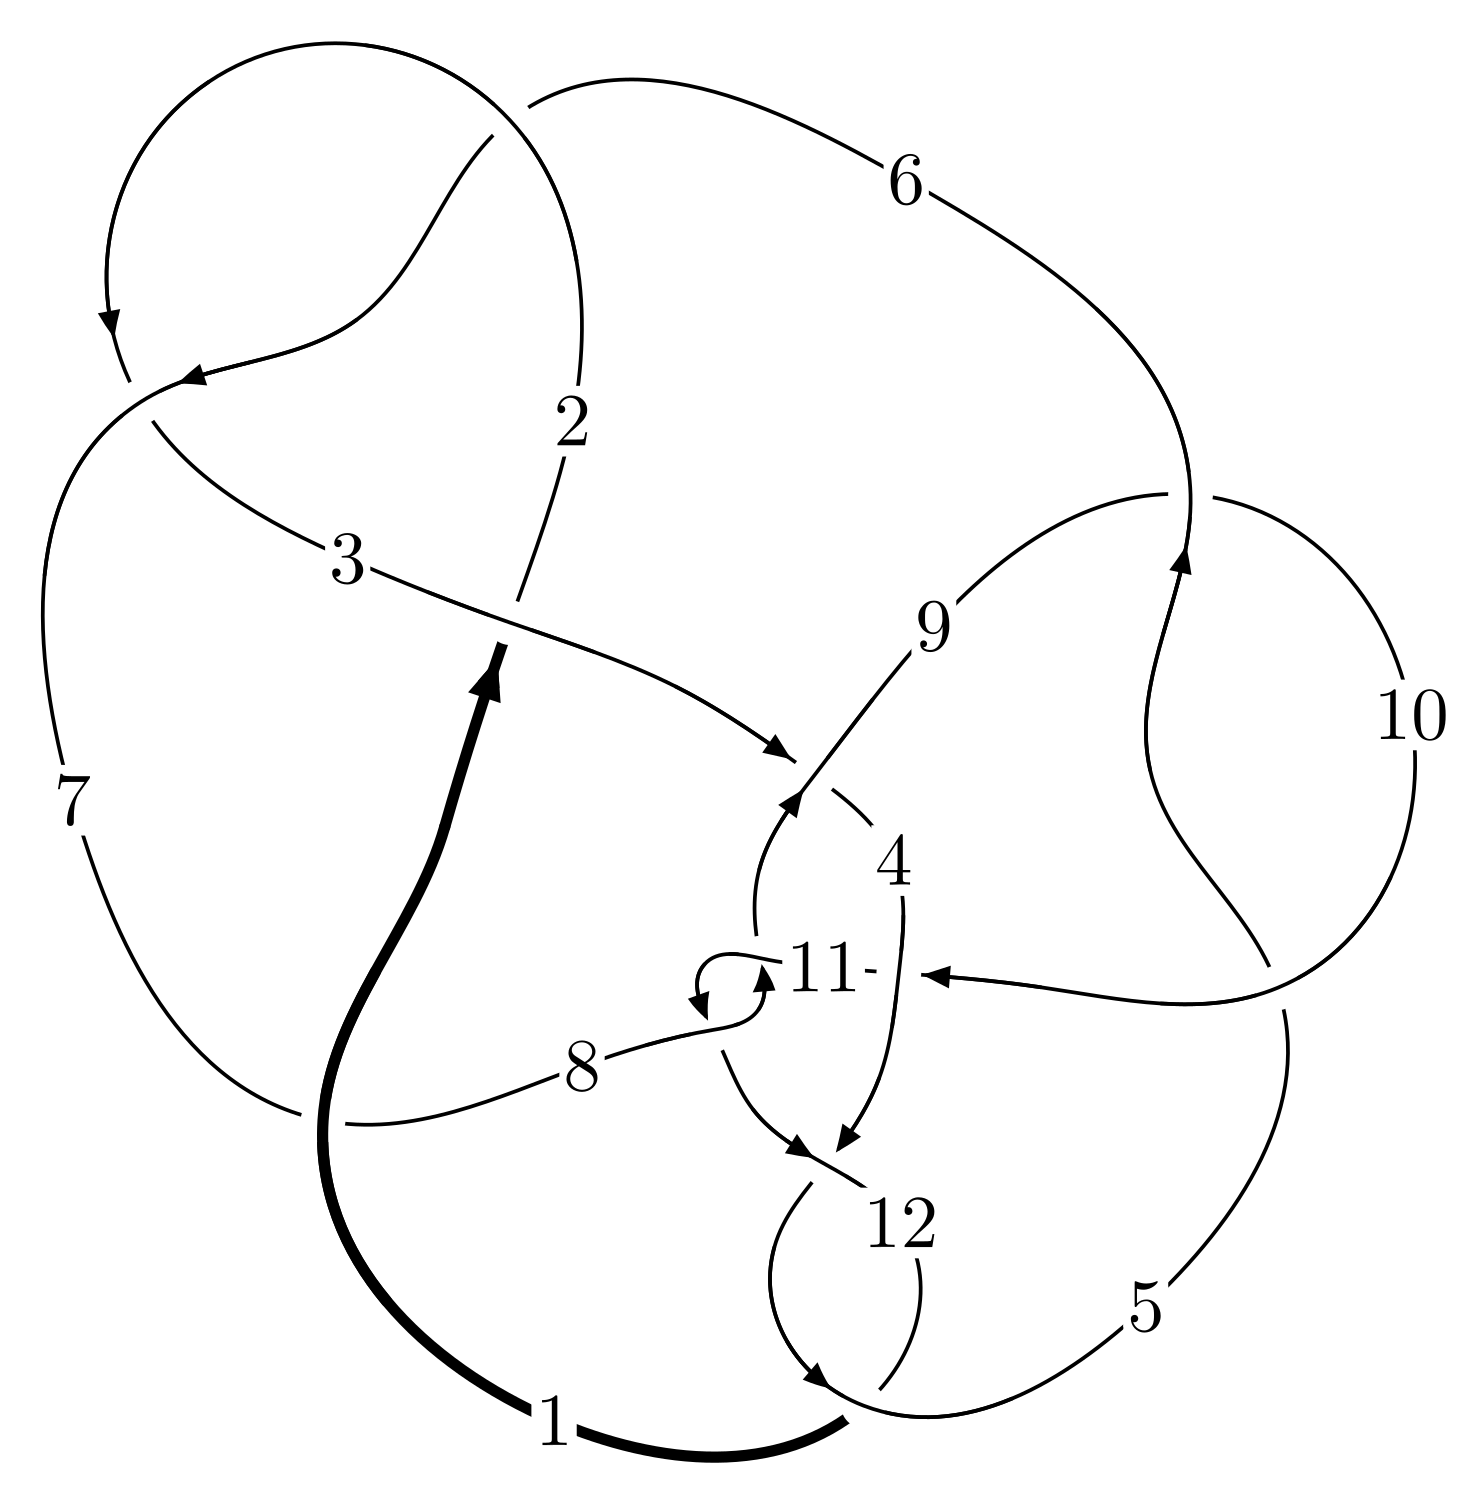
\includegraphics[width=112pt]{../../../GIT/diagram.site/Diagrams/png/1410_12a_0609.png}\\
\ \ \ A knot diagram\footnotemark}&
\allowdisplaybreaks
\textbf{Linearized knot diagam} \\
\cline{2-2}
 &
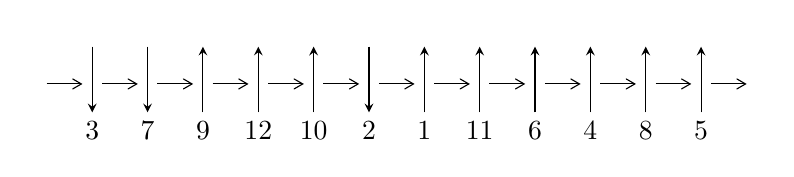
\begin{tikzpicture}[x=20pt, y=17pt]
	% nodes
	\node (C0) at (0, 0) {};
	\node (C1) at (1, 0) {};
	\node (C1U) at (1, +1) {};
	\node (C1D) at (1, -1) {3};

	\node (C2) at (2, 0) {};
	\node (C2U) at (2, +1) {};
	\node (C2D) at (2, -1) {7};

	\node (C3) at (3, 0) {};
	\node (C3U) at (3, +1) {};
	\node (C3D) at (3, -1) {9};

	\node (C4) at (4, 0) {};
	\node (C4U) at (4, +1) {};
	\node (C4D) at (4, -1) {12};

	\node (C5) at (5, 0) {};
	\node (C5U) at (5, +1) {};
	\node (C5D) at (5, -1) {10};

	\node (C6) at (6, 0) {};
	\node (C6U) at (6, +1) {};
	\node (C6D) at (6, -1) {2};

	\node (C7) at (7, 0) {};
	\node (C7U) at (7, +1) {};
	\node (C7D) at (7, -1) {1};

	\node (C8) at (8, 0) {};
	\node (C8U) at (8, +1) {};
	\node (C8D) at (8, -1) {11};

	\node (C9) at (9, 0) {};
	\node (C9U) at (9, +1) {};
	\node (C9D) at (9, -1) {6};

	\node (C10) at (10, 0) {};
	\node (C10U) at (10, +1) {};
	\node (C10D) at (10, -1) {4};

	\node (C11) at (11, 0) {};
	\node (C11U) at (11, +1) {};
	\node (C11D) at (11, -1) {8};

	\node (C12) at (12, 0) {};
	\node (C12U) at (12, +1) {};
	\node (C12D) at (12, -1) {5};
	\node (C13) at (13, 0) {};

	% arrows
	\draw[->,>={angle 60}]
	(C0) edge (C1) (C1) edge (C2) (C2) edge (C3) (C3) edge (C4) (C4) edge (C5) (C5) edge (C6) (C6) edge (C7) (C7) edge (C8) (C8) edge (C9) (C9) edge (C10) (C10) edge (C11) (C11) edge (C12) (C12) edge (C13) ;	\draw[->,>=stealth]
	(C1U) edge (C1D) (C2U) edge (C2D) (C3D) edge (C3U) (C4D) edge (C4U) (C5D) edge (C5U) (C6U) edge (C6D) (C7D) edge (C7U) (C8D) edge (C8U) (C9D) edge (C9U) (C10D) edge (C10U) (C11D) edge (C11U) (C12D) edge (C12U) ;
	\end{tikzpicture} \\
\hhline{~~} \\& 
\textbf{Solving Sequence} \\ \cline{2-2} 
 &
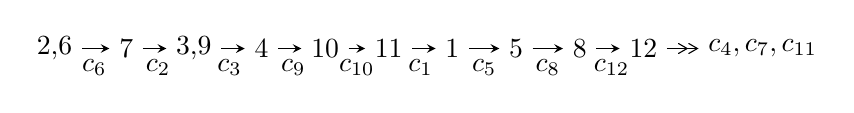
\begin{tikzpicture}[x=23pt, y=7pt]
	% node
	\node (A0) at (-1/8, 0) {2,6};
	\node (A1) at (1, 0) {7};
	\node (A2) at (33/16, 0) {3,9};
	\node (A3) at (25/8, 0) {4};
	\node (A4) at (33/8, 0) {10};
	\node (A5) at (41/8, 0) {11};
	\node (A6) at (49/8, 0) {1};
	\node (A7) at (57/8, 0) {5};
	\node (A8) at (65/8, 0) {8};
	\node (A9) at (73/8, 0) {12};
	\node (C1) at (1/2, -1) {$c_{6}$};
	\node (C2) at (3/2, -1) {$c_{2}$};
	\node (C3) at (21/8, -1) {$c_{3}$};
	\node (C4) at (29/8, -1) {$c_{9}$};
	\node (C5) at (37/8, -1) {$c_{10}$};
	\node (C6) at (45/8, -1) {$c_{1}$};
	\node (C7) at (53/8, -1) {$c_{5}$};
	\node (C8) at (61/8, -1) {$c_{8}$};
	\node (C9) at (69/8, -1) {$c_{12}$};
	\node (A10) at (11, 0) {$c_{4},c_{7},c_{11}$};

	% edge
	\draw[->,>=stealth]	
	(A0) edge (A1) (A1) edge (A2) (A2) edge (A3) (A3) edge (A4) (A4) edge (A5) (A5) edge (A6) (A6) edge (A7) (A7) edge (A8) (A8) edge (A9) ;
	\draw[->>,>={angle 60}]	
	(A9) edge (A10);
\end{tikzpicture} \\ 

\end{tabular} \\

\footnotetext{
The image of knot diagram is generated by the software ``\textbf{Draw programme}" developed by Andrew Bartholomew(\url{http://www.layer8.co.uk/maths/draw/index.htm\#Running-draw}), where we modified some parts for our purpose(\url{https://github.com/CATsTAILs/LinksPainter}).
}\phantom \\ \newline 
\centering \textbf{Ideals for irreducible components\footnotemark of $X_{\text{par}}$} 
 
\begin{align*}
I^u_{1}&=\langle 
-7.11550\times10^{270} u^{147}+2.34975\times10^{270} u^{146}+\cdots+7.83329\times10^{269} b+1.17176\times10^{272},\\
\phantom{I^u_{1}}&\phantom{= \langle  }2.42818\times10^{272} u^{147}-8.26249\times10^{271} u^{146}+\cdots+8.61662\times10^{270} a-3.99086\times10^{273},\\
\phantom{I^u_{1}}&\phantom{= \langle  }u^{148}- u^{147}+\cdots-28 u+11\rangle \\
I^u_{2}&=\langle 
u^{36}-6 u^{35}+\cdots+b+5,\;-28 u^{36}+22 u^{35}+\cdots+a-30,\;u^{37}-10 u^{35}+\cdots-7 u^2+1\rangle \\
\\
\end{align*}
\raggedright * 2 irreducible components of $\dim_{\mathbb{C}}=0$, with total 185 representations.\\
\footnotetext{All coefficients of polynomials are rational numbers. But the coefficients are sometimes approximated in decimal forms when there is not enough margin.}
\newpage
\renewcommand{\arraystretch}{1}
\centering \section*{I. $I^u_{1}= \langle -7.12\times10^{270} u^{147}+2.35\times10^{270} u^{146}+\cdots+7.83\times10^{269} b+1.17\times10^{272},\;2.43\times10^{272} u^{147}-8.26\times10^{271} u^{146}+\cdots+8.62\times10^{270} a-3.99\times10^{273},\;u^{148}- u^{147}+\cdots-28 u+11 \rangle$}
\flushleft \textbf{(i) Arc colorings}\\
\begin{tabular}{m{7pt} m{180pt} m{7pt} m{180pt} }
\flushright $a_{2}=$&$\begin{pmatrix}0\\u\end{pmatrix}$ \\
\flushright $a_{6}=$&$\begin{pmatrix}1\\0\end{pmatrix}$ \\
\flushright $a_{7}=$&$\begin{pmatrix}1\\u^2\end{pmatrix}$ \\
\flushright $a_{3}=$&$\begin{pmatrix}- u\\- u^3+u\end{pmatrix}$ \\
\flushright $a_{9}=$&$\begin{pmatrix}-28.1802 u^{147}+9.58902 u^{146}+\cdots-500.278 u+463.158\\9.08367 u^{147}-2.99969 u^{146}+\cdots+149.153 u-149.588\end{pmatrix}$ \\
\flushright $a_{4}=$&$\begin{pmatrix}28.9466 u^{147}-7.64764 u^{146}+\cdots+511.326 u-413.056\\1.87191 u^{147}+0.474465 u^{146}+\cdots+37.3094 u-3.29970\end{pmatrix}$ \\
\flushright $a_{10}=$&$\begin{pmatrix}-19.0965 u^{147}+6.58932 u^{146}+\cdots-351.125 u+313.570\\9.08367 u^{147}-2.99969 u^{146}+\cdots+149.153 u-149.588\end{pmatrix}$ \\
\flushright $a_{11}=$&$\begin{pmatrix}-1.63584 u^{147}+2.74753 u^{146}+\cdots-9.74895 u+59.5619\\9.74060 u^{147}-3.27722 u^{146}+\cdots+170.925 u-160.730\end{pmatrix}$ \\
\flushright $a_{1}=$&$\begin{pmatrix}u^3\\u^5- u^3+u\end{pmatrix}$ \\
\flushright $a_{5}=$&$\begin{pmatrix}19.2042 u^{147}-3.52906 u^{146}+\cdots+360.206 u-255.473\\-15.6776 u^{147}+5.49972 u^{146}+\cdots-272.591 u+266.188\end{pmatrix}$ \\
\flushright $a_{8}=$&$\begin{pmatrix}u^6- u^4+1\\u^8-2 u^6+2 u^4\end{pmatrix}$ \\
\flushright $a_{12}=$&$\begin{pmatrix}-4.32037 u^{147}+0.0334826 u^{146}+\cdots-91.4009 u+53.4061\\-10.0898 u^{147}+3.69835 u^{146}+\cdots-173.459 u+173.267\end{pmatrix}$\\&\end{tabular}
\flushleft \textbf{(ii) Obstruction class $= -1$}\\~\\
\flushleft \textbf{(iii) Cusp Shapes $= 170.660 u^{147}-53.4676 u^{146}+\cdots+2947.57 u-2741.52$}\\~\\
\newpage\renewcommand{\arraystretch}{1}
\flushleft \textbf{(iv) u-Polynomials at the component}\newline \\
\begin{tabular}{m{50pt}|m{274pt}}
Crossings & \hspace{64pt}u-Polynomials at each crossing \\
\hline $$\begin{aligned}c_{1}\end{aligned}$$&$\begin{aligned}
&u^{148}+77 u^{147}+\cdots+2082 u+121
\end{aligned}$\\
\hline $$\begin{aligned}c_{2},c_{6}\end{aligned}$$&$\begin{aligned}
&u^{148}- u^{147}+\cdots-28 u+11
\end{aligned}$\\
\hline $$\begin{aligned}c_{3}\end{aligned}$$&$\begin{aligned}
&u^{148}- u^{147}+\cdots-437764162 u+31663951
\end{aligned}$\\
\hline $$\begin{aligned}c_{4},c_{12}\end{aligned}$$&$\begin{aligned}
&u^{148}-41 u^{146}+\cdots-1867 u-457
\end{aligned}$\\
\hline $$\begin{aligned}c_{5},c_{9}\end{aligned}$$&$\begin{aligned}
&u^{148}-2 u^{147}+\cdots-20681 u-4913
\end{aligned}$\\
\hline $$\begin{aligned}c_{7}\end{aligned}$$&$\begin{aligned}
&u^{148}-3 u^{147}+\cdots-52130042 u+4546267
\end{aligned}$\\
\hline $$\begin{aligned}c_{8},c_{11}\end{aligned}$$&$\begin{aligned}
&u^{148}+6 u^{147}+\cdots+147861 u+10043
\end{aligned}$\\
\hline $$\begin{aligned}c_{10}\end{aligned}$$&$\begin{aligned}
&u^{148}+u^{147}+\cdots-171710 u-36269
\end{aligned}$\\
\hline
\end{tabular}\\~\\
\newpage\renewcommand{\arraystretch}{1}
\flushleft \textbf{(v) Riley Polynomials at the component}\newline \\
\begin{tabular}{m{50pt}|m{274pt}}
Crossings & \hspace{64pt}Riley Polynomials at each crossing \\
\hline $$\begin{aligned}c_{1}\end{aligned}$$&$\begin{aligned}
&y^{148}-5 y^{147}+\cdots-428602 y+14641
\end{aligned}$\\
\hline $$\begin{aligned}c_{2},c_{6}\end{aligned}$$&$\begin{aligned}
&y^{148}-77 y^{147}+\cdots-2082 y+121
\end{aligned}$\\
\hline $$\begin{aligned}c_{3}\end{aligned}$$&$\begin{aligned}
&y^{148}+59 y^{147}+\cdots-106286132462952552 y+1002605792930401
\end{aligned}$\\
\hline $$\begin{aligned}c_{4},c_{12}\end{aligned}$$&$\begin{aligned}
&y^{148}-82 y^{147}+\cdots-21312345 y+208849
\end{aligned}$\\
\hline $$\begin{aligned}c_{5},c_{9}\end{aligned}$$&$\begin{aligned}
&y^{148}+98 y^{147}+\cdots+311191787 y+24137569
\end{aligned}$\\
\hline $$\begin{aligned}c_{7}\end{aligned}$$&$\begin{aligned}
&y^{148}+87 y^{147}+\cdots+203578457803668 y+20668543635289
\end{aligned}$\\
\hline $$\begin{aligned}c_{8},c_{11}\end{aligned}$$&$\begin{aligned}
&y^{148}+90 y^{147}+\cdots+2708328479 y+100861849
\end{aligned}$\\
\hline $$\begin{aligned}c_{10}\end{aligned}$$&$\begin{aligned}
&y^{148}+23 y^{147}+\cdots-9866857228 y+1315440361
\end{aligned}$\\
\hline
\end{tabular}\\~\\
\newpage\flushleft \textbf{(vi) Complex Volumes and Cusp Shapes}
$$\begin{array}{c|c|c}  
\text{Solutions to }I^u_{1}& \I (\text{vol} + \sqrt{-1}CS) & \text{Cusp shape}\\
 \hline 
\begin{aligned}
u &= -0.801882 + 0.564876 I \\
a &= -1.98309 - 1.20150 I \\
b &= \phantom{-}0.201767 + 1.107530 I\end{aligned}
 & -4.17373 + 5.78306 I & \phantom{-0.000000 } 0 \\ \hline\begin{aligned}
u &= -0.801882 - 0.564876 I \\
a &= -1.98309 + 1.20150 I \\
b &= \phantom{-}0.201767 - 1.107530 I\end{aligned}
 & -4.17373 - 5.78306 I & \phantom{-0.000000 } 0 \\ \hline\begin{aligned}
u &= \phantom{-}0.753591 + 0.626874 I \\
a &= \phantom{-}0.185539 - 1.185390 I \\
b &= \phantom{-}0.497327 + 0.904516 I\end{aligned}
 & \phantom{-}2.94244 + 1.46559 I & \phantom{-0.000000 } 0 \\ \hline\begin{aligned}
u &= \phantom{-}0.753591 - 0.626874 I \\
a &= \phantom{-}0.185539 + 1.185390 I \\
b &= \phantom{-}0.497327 - 0.904516 I\end{aligned}
 & \phantom{-}2.94244 - 1.46559 I & \phantom{-0.000000 } 0 \\ \hline\begin{aligned}
u &= \phantom{-}0.819922 + 0.622130 I \\
a &= \phantom{-}1.49093 - 0.46144 I \\
b &= -0.591941 + 1.046700 I\end{aligned}
 & \phantom{-}2.73613 - 6.32545 I & \phantom{-0.000000 } 0 \\ \hline\begin{aligned}
u &= \phantom{-}0.819922 - 0.622130 I \\
a &= \phantom{-}1.49093 + 0.46144 I \\
b &= -0.591941 - 1.046700 I\end{aligned}
 & \phantom{-}2.73613 + 6.32545 I & \phantom{-0.000000 } 0 \\ \hline\begin{aligned}
u &= \phantom{-}0.949221 + 0.199178 I \\
a &= -1.89330 - 0.09556 I \\
b &= \phantom{-}0.727956 - 0.713865 I\end{aligned}
 & -3.20129 - 5.06040 I & \phantom{-0.000000 } 0 \\ \hline\begin{aligned}
u &= \phantom{-}0.949221 - 0.199178 I \\
a &= -1.89330 + 0.09556 I \\
b &= \phantom{-}0.727956 + 0.713865 I\end{aligned}
 & -3.20129 + 5.06040 I & \phantom{-0.000000 } 0 \\ \hline\begin{aligned}
u &= -0.965652 + 0.381043 I \\
a &= -0.082316 + 0.291581 I \\
b &= \phantom{-}0.278548 - 0.430341 I\end{aligned}
 & -1.50408 + 1.47661 I & \phantom{-0.000000 } 0 \\ \hline\begin{aligned}
u &= -0.965652 - 0.381043 I \\
a &= -0.082316 - 0.291581 I \\
b &= \phantom{-}0.278548 + 0.430341 I\end{aligned}
 & -1.50408 - 1.47661 I & \phantom{-0.000000 } 0\\
 \hline 
 \end{array}$$\newpage$$\begin{array}{c|c|c}  
\text{Solutions to }I^u_{1}& \I (\text{vol} + \sqrt{-1}CS) & \text{Cusp shape}\\
 \hline 
\begin{aligned}
u &= -1.032450 + 0.117025 I \\
a &= -0.356571 - 0.269265 I \\
b &= \phantom{-}0.461349 + 0.517094 I\end{aligned}
 & -3.46852 - 0.71657 I & \phantom{-0.000000 } 0 \\ \hline\begin{aligned}
u &= -1.032450 - 0.117025 I \\
a &= -0.356571 + 0.269265 I \\
b &= \phantom{-}0.461349 - 0.517094 I\end{aligned}
 & -3.46852 + 0.71657 I & \phantom{-0.000000 } 0 \\ \hline\begin{aligned}
u &= -0.722106 + 0.626635 I \\
a &= -1.101530 + 0.062706 I \\
b &= \phantom{-}0.826797 - 0.355727 I\end{aligned}
 & \phantom{-}1.99222 + 6.26430 I & \phantom{-0.000000 } 0 \\ \hline\begin{aligned}
u &= -0.722106 - 0.626635 I \\
a &= -1.101530 - 0.062706 I \\
b &= \phantom{-}0.826797 + 0.355727 I\end{aligned}
 & \phantom{-}1.99222 - 6.26430 I & \phantom{-0.000000 } 0 \\ \hline\begin{aligned}
u &= -0.918255 + 0.497223 I \\
a &= -1.42108 + 1.16642 I \\
b &= \phantom{-}0.861920 + 0.742199 I\end{aligned}
 & \phantom{-}3.60069 + 3.57734 I & \phantom{-0.000000 } 0 \\ \hline\begin{aligned}
u &= -0.918255 - 0.497223 I \\
a &= -1.42108 - 1.16642 I \\
b &= \phantom{-}0.861920 - 0.742199 I\end{aligned}
 & \phantom{-}3.60069 - 3.57734 I & \phantom{-0.000000 } 0 \\ \hline\begin{aligned}
u &= \phantom{-}0.950293 + 0.434823 I \\
a &= -1.34910 - 0.73463 I \\
b &= \phantom{-}0.557261 - 0.168149 I\end{aligned}
 & -0.39596 - 3.88277 I & \phantom{-0.000000 } 0 \\ \hline\begin{aligned}
u &= \phantom{-}0.950293 - 0.434823 I \\
a &= -1.34910 + 0.73463 I \\
b &= \phantom{-}0.557261 + 0.168149 I\end{aligned}
 & -0.39596 + 3.88277 I & \phantom{-0.000000 } 0 \\ \hline\begin{aligned}
u &= -0.448329 + 0.840026 I \\
a &= \phantom{-}0.421644 - 0.849882 I \\
b &= -0.194488 + 1.268240 I\end{aligned}
 & -2.82616 - 2.12943 I & \phantom{-0.000000 } 0 \\ \hline\begin{aligned}
u &= -0.448329 - 0.840026 I \\
a &= \phantom{-}0.421644 + 0.849882 I \\
b &= -0.194488 - 1.268240 I\end{aligned}
 & -2.82616 + 2.12943 I & \phantom{-0.000000 } 0\\
 \hline 
 \end{array}$$\newpage$$\begin{array}{c|c|c}  
\text{Solutions to }I^u_{1}& \I (\text{vol} + \sqrt{-1}CS) & \text{Cusp shape}\\
 \hline 
\begin{aligned}
u &= -0.333726 + 1.007330 I \\
a &= -0.120235 + 0.741241 I \\
b &= \phantom{-}0.095350 - 1.282620 I\end{aligned}
 & -3.75918 - 2.82637 I & \phantom{-0.000000 } 0 \\ \hline\begin{aligned}
u &= -0.333726 - 1.007330 I \\
a &= -0.120235 - 0.741241 I \\
b &= \phantom{-}0.095350 + 1.282620 I\end{aligned}
 & -3.75918 + 2.82637 I & \phantom{-0.000000 } 0 \\ \hline\begin{aligned}
u &= -0.859504 + 0.623047 I \\
a &= \phantom{-}1.11434 - 0.94865 I \\
b &= -0.602274 - 0.505888 I\end{aligned}
 & \phantom{-}1.60311 - 1.40810 I & \phantom{-0.000000 } 0 \\ \hline\begin{aligned}
u &= -0.859504 - 0.623047 I \\
a &= \phantom{-}1.11434 + 0.94865 I \\
b &= -0.602274 + 0.505888 I\end{aligned}
 & \phantom{-}1.60311 + 1.40810 I & \phantom{-0.000000 } 0 \\ \hline\begin{aligned}
u &= \phantom{-}0.115334 + 1.057600 I \\
a &= -0.279424 - 0.411326 I \\
b &= \phantom{-}0.031526 + 1.026900 I\end{aligned}
 & -4.73792 + 0.18945 I & \phantom{-0.000000 } 0 \\ \hline\begin{aligned}
u &= \phantom{-}0.115334 - 1.057600 I \\
a &= -0.279424 + 0.411326 I \\
b &= \phantom{-}0.031526 - 1.026900 I\end{aligned}
 & -4.73792 - 0.18945 I & \phantom{-0.000000 } 0 \\ \hline\begin{aligned}
u &= \phantom{-}0.247947 + 0.901431 I \\
a &= -1.116440 - 0.780764 I \\
b &= \phantom{-}0.57458 + 1.36111 I\end{aligned}
 & -4.3204 + 13.9557 I & \phantom{-0.000000 } 0 \\ \hline\begin{aligned}
u &= \phantom{-}0.247947 - 0.901431 I \\
a &= -1.116440 + 0.780764 I \\
b &= \phantom{-}0.57458 - 1.36111 I\end{aligned}
 & -4.3204 - 13.9557 I & \phantom{-0.000000 } 0 \\ \hline\begin{aligned}
u &= -0.724944 + 0.522800 I \\
a &= \phantom{-}1.18389 + 0.92493 I \\
b &= -0.176138 - 0.961064 I\end{aligned}
 & -1.19364 + 2.08514 I & \phantom{-0.000000 } 0 \\ \hline\begin{aligned}
u &= -0.724944 - 0.522800 I \\
a &= \phantom{-}1.18389 - 0.92493 I \\
b &= -0.176138 + 0.961064 I\end{aligned}
 & -1.19364 - 2.08514 I & \phantom{-0.000000 } 0\\
 \hline 
 \end{array}$$\newpage$$\begin{array}{c|c|c}  
\text{Solutions to }I^u_{1}& \I (\text{vol} + \sqrt{-1}CS) & \text{Cusp shape}\\
 \hline 
\begin{aligned}
u &= -0.759102 + 0.461625 I \\
a &= -0.32697 - 1.90410 I \\
b &= \phantom{-}0.047807 + 1.073240 I\end{aligned}
 & -4.01726 - 1.52458 I & \phantom{-0.000000 } 0 \\ \hline\begin{aligned}
u &= -0.759102 - 0.461625 I \\
a &= -0.32697 + 1.90410 I \\
b &= \phantom{-}0.047807 - 1.073240 I\end{aligned}
 & -4.01726 + 1.52458 I & \phantom{-0.000000 } 0 \\ \hline\begin{aligned}
u &= -0.996847 + 0.518156 I \\
a &= -0.515323 + 0.715296 I \\
b &= \phantom{-}0.575549 - 0.924658 I\end{aligned}
 & -1.260890 + 0.226294 I & \phantom{-0.000000 } 0 \\ \hline\begin{aligned}
u &= -0.996847 - 0.518156 I \\
a &= -0.515323 - 0.715296 I \\
b &= \phantom{-}0.575549 + 0.924658 I\end{aligned}
 & -1.260890 - 0.226294 I & \phantom{-0.000000 } 0 \\ \hline\begin{aligned}
u &= -1.115870 + 0.152069 I \\
a &= -0.241236 - 0.379829 I \\
b &= -0.051143 - 1.079750 I\end{aligned}
 & -2.92928 + 2.44675 I & \phantom{-0.000000 } 0 \\ \hline\begin{aligned}
u &= -1.115870 - 0.152069 I \\
a &= -0.241236 + 0.379829 I \\
b &= -0.051143 + 1.079750 I\end{aligned}
 & -2.92928 - 2.44675 I & \phantom{-0.000000 } 0 \\ \hline\begin{aligned}
u &= \phantom{-}1.083390 + 0.374604 I \\
a &= \phantom{-}0.677527 + 0.958052 I \\
b &= \phantom{-}0.18251 + 1.54932 I\end{aligned}
 & -6.85236 + 0.13574 I & \phantom{-0.000000 } 0 \\ \hline\begin{aligned}
u &= \phantom{-}1.083390 - 0.374604 I \\
a &= \phantom{-}0.677527 - 0.958052 I \\
b &= \phantom{-}0.18251 - 1.54932 I\end{aligned}
 & -6.85236 - 0.13574 I & \phantom{-0.000000 } 0 \\ \hline\begin{aligned}
u &= \phantom{-}0.204334 + 0.826121 I \\
a &= \phantom{-}1.124900 + 0.715403 I \\
b &= -0.61938 - 1.35395 I\end{aligned}
 & -0.51756 + 7.81284 I & \phantom{-0.000000 } 0 \\ \hline\begin{aligned}
u &= \phantom{-}0.204334 - 0.826121 I \\
a &= \phantom{-}1.124900 - 0.715403 I \\
b &= -0.61938 + 1.35395 I\end{aligned}
 & -0.51756 - 7.81284 I & \phantom{-0.000000 } 0\\
 \hline 
 \end{array}$$\newpage$$\begin{array}{c|c|c}  
\text{Solutions to }I^u_{1}& \I (\text{vol} + \sqrt{-1}CS) & \text{Cusp shape}\\
 \hline 
\begin{aligned}
u &= \phantom{-}1.113590 + 0.291888 I \\
a &= \phantom{-}0.293297 + 1.021440 I \\
b &= \phantom{-}0.159837 + 1.392530 I\end{aligned}
 & -7.03383 + 0.08971 I & \phantom{-0.000000 } 0 \\ \hline\begin{aligned}
u &= \phantom{-}1.113590 - 0.291888 I \\
a &= \phantom{-}0.293297 - 1.021440 I \\
b &= \phantom{-}0.159837 - 1.392530 I\end{aligned}
 & -7.03383 - 0.08971 I & \phantom{-0.000000 } 0 \\ \hline\begin{aligned}
u &= \phantom{-}0.432270 + 0.720324 I \\
a &= \phantom{-}0.611532 - 1.000840 I \\
b &= -0.286130 + 0.372349 I\end{aligned}
 & \phantom{-}1.19324 + 2.46533 I & \phantom{-0.000000 } 0 \\ \hline\begin{aligned}
u &= \phantom{-}0.432270 - 0.720324 I \\
a &= \phantom{-}0.611532 + 1.000840 I \\
b &= -0.286130 - 0.372349 I\end{aligned}
 & \phantom{-}1.19324 - 2.46533 I & \phantom{-0.000000 } 0 \\ \hline\begin{aligned}
u &= -0.210776 + 0.813138 I \\
a &= -1.45325 + 0.79425 I \\
b &= \phantom{-}0.439344 - 1.255070 I\end{aligned}
 & -7.18334 - 7.02861 I & \phantom{-0.000000 } 0 \\ \hline\begin{aligned}
u &= -0.210776 - 0.813138 I \\
a &= -1.45325 - 0.79425 I \\
b &= \phantom{-}0.439344 + 1.255070 I\end{aligned}
 & -7.18334 + 7.02861 I & \phantom{-0.000000 } 0 \\ \hline\begin{aligned}
u &= \phantom{-}0.781945 + 0.857312 I \\
a &= -0.101971 + 0.902087 I \\
b &= -0.312973 - 1.056760 I\end{aligned}
 & -0.06242 + 4.94279 I & \phantom{-0.000000 } 0 \\ \hline\begin{aligned}
u &= \phantom{-}0.781945 - 0.857312 I \\
a &= -0.101971 - 0.902087 I \\
b &= -0.312973 + 1.056760 I\end{aligned}
 & -0.06242 - 4.94279 I & \phantom{-0.000000 } 0 \\ \hline\begin{aligned}
u &= \phantom{-}0.026933 + 0.836326 I \\
a &= -1.049010 - 0.576149 I \\
b &= \phantom{-}0.625028 + 1.186720 I\end{aligned}
 & -6.07873 + 2.17643 I & \phantom{-0.000000 } 0 \\ \hline\begin{aligned}
u &= \phantom{-}0.026933 - 0.836326 I \\
a &= -1.049010 + 0.576149 I \\
b &= \phantom{-}0.625028 - 1.186720 I\end{aligned}
 & -6.07873 - 2.17643 I & \phantom{-0.000000 } 0\\
 \hline 
 \end{array}$$\newpage$$\begin{array}{c|c|c}  
\text{Solutions to }I^u_{1}& \I (\text{vol} + \sqrt{-1}CS) & \text{Cusp shape}\\
 \hline 
\begin{aligned}
u &= -1.089850 + 0.408220 I \\
a &= \phantom{-}0.637757 - 0.676371 I \\
b &= -0.700513 + 0.898650 I\end{aligned}
 & -1.29393 + 0.96563 I & \phantom{-0.000000 } 0 \\ \hline\begin{aligned}
u &= -1.089850 - 0.408220 I \\
a &= \phantom{-}0.637757 + 0.676371 I \\
b &= -0.700513 - 0.898650 I\end{aligned}
 & -1.29393 - 0.96563 I & \phantom{-0.000000 } 0 \\ \hline\begin{aligned}
u &= \phantom{-}1.100130 + 0.385626 I \\
a &= \phantom{-}1.40067 + 2.02165 I \\
b &= \phantom{-}0.032025 + 1.022240 I\end{aligned}
 & -3.99476 + 2.05581 I & \phantom{-0.000000 } 0 \\ \hline\begin{aligned}
u &= \phantom{-}1.100130 - 0.385626 I \\
a &= \phantom{-}1.40067 - 2.02165 I \\
b &= \phantom{-}0.032025 - 1.022240 I\end{aligned}
 & -3.99476 - 2.05581 I & \phantom{-0.000000 } 0 \\ \hline\begin{aligned}
u &= \phantom{-}0.875901 + 0.772682 I \\
a &= -1.274370 + 0.495646 I \\
b &= \phantom{-}0.439542 - 1.121260 I\end{aligned}
 & -0.39615 - 10.89840 I & \phantom{-0.000000 } 0 \\ \hline\begin{aligned}
u &= \phantom{-}0.875901 - 0.772682 I \\
a &= -1.274370 - 0.495646 I \\
b &= \phantom{-}0.439542 + 1.121260 I\end{aligned}
 & -0.39615 + 10.89840 I & \phantom{-0.000000 } 0 \\ \hline\begin{aligned}
u &= \phantom{-}0.492360 + 0.668072 I \\
a &= \phantom{-}1.000830 + 0.736488 I \\
b &= -0.436862 - 0.283519 I\end{aligned}
 & \phantom{-}1.53421 - 0.23768 I & \phantom{-0.000000 } 0 \\ \hline\begin{aligned}
u &= \phantom{-}0.492360 - 0.668072 I \\
a &= \phantom{-}1.000830 - 0.736488 I \\
b &= -0.436862 + 0.283519 I\end{aligned}
 & \phantom{-}1.53421 + 0.23768 I & \phantom{-0.000000 } 0 \\ \hline\begin{aligned}
u &= \phantom{-}1.047440 + 0.555613 I \\
a &= -1.087820 - 0.185331 I \\
b &= \phantom{-}0.478821 - 0.312236 I\end{aligned}
 & -0.11027 - 4.51657 I & \phantom{-0.000000 } 0 \\ \hline\begin{aligned}
u &= \phantom{-}1.047440 - 0.555613 I \\
a &= -1.087820 + 0.185331 I \\
b &= \phantom{-}0.478821 + 0.312236 I\end{aligned}
 & -0.11027 + 4.51657 I & \phantom{-0.000000 } 0\\
 \hline 
 \end{array}$$\newpage$$\begin{array}{c|c|c}  
\text{Solutions to }I^u_{1}& \I (\text{vol} + \sqrt{-1}CS) & \text{Cusp shape}\\
 \hline 
\begin{aligned}
u &= \phantom{-}0.433187 + 0.680149 I \\
a &= \phantom{-}0.528844 + 1.295920 I \\
b &= \phantom{-}0.022821 - 0.691902 I\end{aligned}
 & \phantom{-}1.67106 - 0.48268 I & \phantom{-0.000000 } 0 \\ \hline\begin{aligned}
u &= \phantom{-}0.433187 - 0.680149 I \\
a &= \phantom{-}0.528844 - 1.295920 I \\
b &= \phantom{-}0.022821 + 0.691902 I\end{aligned}
 & \phantom{-}1.67106 + 0.48268 I & \phantom{-0.000000 } 0 \\ \hline\begin{aligned}
u &= -0.240264 + 0.766217 I \\
a &= -1.68880 + 0.13667 I \\
b &= \phantom{-}1.163530 + 0.077343 I\end{aligned}
 & -0.25443 - 7.84410 I & \phantom{-0.000000 } 0 \\ \hline\begin{aligned}
u &= -0.240264 - 0.766217 I \\
a &= -1.68880 - 0.13667 I \\
b &= \phantom{-}1.163530 - 0.077343 I\end{aligned}
 & -0.25443 + 7.84410 I & \phantom{-0.000000 } 0 \\ \hline\begin{aligned}
u &= \phantom{-}1.129290 + 0.397204 I \\
a &= -0.59756 - 1.42716 I \\
b &= \phantom{-}1.333640 - 0.128607 I\end{aligned}
 & -0.28445 - 2.28003 I & \phantom{-0.000000 } 0 \\ \hline\begin{aligned}
u &= \phantom{-}1.129290 - 0.397204 I \\
a &= -0.59756 + 1.42716 I \\
b &= \phantom{-}1.333640 + 0.128607 I\end{aligned}
 & -0.28445 + 2.28003 I & \phantom{-0.000000 } 0 \\ \hline\begin{aligned}
u &= -0.630802 + 0.496059 I \\
a &= \phantom{-}1.212270 - 0.453506 I \\
b &= -1.040690 + 0.562959 I\end{aligned}
 & \phantom{-}4.44277 + 0.54060 I & \phantom{-0.000000 } 0 \\ \hline\begin{aligned}
u &= -0.630802 - 0.496059 I \\
a &= \phantom{-}1.212270 + 0.453506 I \\
b &= -1.040690 - 0.562959 I\end{aligned}
 & \phantom{-}4.44277 - 0.54060 I & \phantom{-0.000000 } 0 \\ \hline\begin{aligned}
u &= \phantom{-}1.158480 + 0.321521 I \\
a &= \phantom{-}0.330875 + 0.959728 I \\
b &= -1.147530 - 0.154773 I\end{aligned}
 & -4.43528 + 4.50982 I & \phantom{-0.000000 } 0 \\ \hline\begin{aligned}
u &= \phantom{-}1.158480 - 0.321521 I \\
a &= \phantom{-}0.330875 - 0.959728 I \\
b &= -1.147530 + 0.154773 I\end{aligned}
 & -4.43528 - 4.50982 I & \phantom{-0.000000 } 0\\
 \hline 
 \end{array}$$\newpage$$\begin{array}{c|c|c}  
\text{Solutions to }I^u_{1}& \I (\text{vol} + \sqrt{-1}CS) & \text{Cusp shape}\\
 \hline 
\begin{aligned}
u &= \phantom{-}1.059780 + 0.571412 I \\
a &= -1.35632 + 0.45880 I \\
b &= \phantom{-}0.170067 - 0.674015 I\end{aligned}
 & -0.13946 - 4.36646 I & \phantom{-0.000000 } 0 \\ \hline\begin{aligned}
u &= \phantom{-}1.059780 - 0.571412 I \\
a &= -1.35632 - 0.45880 I \\
b &= \phantom{-}0.170067 + 0.674015 I\end{aligned}
 & -0.13946 + 4.36646 I & \phantom{-0.000000 } 0 \\ \hline\begin{aligned}
u &= \phantom{-}1.106090 + 0.508945 I \\
a &= \phantom{-}1.49832 + 0.02977 I \\
b &= -0.719961 + 0.618121 I\end{aligned}
 & -0.54021 - 6.34086 I & \phantom{-0.000000 } 0 \\ \hline\begin{aligned}
u &= \phantom{-}1.106090 - 0.508945 I \\
a &= \phantom{-}1.49832 - 0.02977 I \\
b &= -0.719961 - 0.618121 I\end{aligned}
 & -0.54021 + 6.34086 I & \phantom{-0.000000 } 0 \\ \hline\begin{aligned}
u &= -1.136940 + 0.443245 I \\
a &= \phantom{-}0.62455 - 1.53720 I \\
b &= -0.152187 - 1.152130 I\end{aligned}
 & -2.37651 + 5.08383 I & \phantom{-0.000000 } 0 \\ \hline\begin{aligned}
u &= -1.136940 - 0.443245 I \\
a &= \phantom{-}0.62455 + 1.53720 I \\
b &= -0.152187 + 1.152130 I\end{aligned}
 & -2.37651 - 5.08383 I & \phantom{-0.000000 } 0 \\ \hline\begin{aligned}
u &= \phantom{-}1.077500 + 0.580475 I \\
a &= \phantom{-}0.184332 - 1.015030 I \\
b &= \phantom{-}0.221785 + 0.414699 I\end{aligned}
 & -0.70142 - 7.44159 I & \phantom{-0.000000 } 0 \\ \hline\begin{aligned}
u &= \phantom{-}1.077500 - 0.580475 I \\
a &= \phantom{-}0.184332 + 1.015030 I \\
b &= \phantom{-}0.221785 - 0.414699 I\end{aligned}
 & -0.70142 + 7.44159 I & \phantom{-0.000000 } 0 \\ \hline\begin{aligned}
u &= -1.117770 + 0.510399 I \\
a &= -1.58452 + 1.63949 I \\
b &= \phantom{-}0.230218 + 1.150580 I\end{aligned}
 & -3.07745 + 9.56188 I & \phantom{-0.000000 } 0 \\ \hline\begin{aligned}
u &= -1.117770 - 0.510399 I \\
a &= -1.58452 - 1.63949 I \\
b &= \phantom{-}0.230218 - 1.150580 I\end{aligned}
 & -3.07745 - 9.56188 I & \phantom{-0.000000 } 0\\
 \hline 
 \end{array}$$\newpage$$\begin{array}{c|c|c}  
\text{Solutions to }I^u_{1}& \I (\text{vol} + \sqrt{-1}CS) & \text{Cusp shape}\\
 \hline 
\begin{aligned}
u &= \phantom{-}1.142330 + 0.454417 I \\
a &= -1.69292 - 1.04413 I \\
b &= \phantom{-}0.056090 - 0.996161 I\end{aligned}
 & -2.28746 - 2.85100 I & \phantom{-0.000000 } 0 \\ \hline\begin{aligned}
u &= \phantom{-}1.142330 - 0.454417 I \\
a &= -1.69292 + 1.04413 I \\
b &= \phantom{-}0.056090 + 0.996161 I\end{aligned}
 & -2.28746 + 2.85100 I & \phantom{-0.000000 } 0 \\ \hline\begin{aligned}
u &= \phantom{-}1.145310 + 0.447419 I \\
a &= -0.768700 - 0.149089 I \\
b &= -0.45578 - 1.63998 I\end{aligned}
 & -8.58012 - 5.99056 I & \phantom{-0.000000 } 0 \\ \hline\begin{aligned}
u &= \phantom{-}1.145310 - 0.447419 I \\
a &= -0.768700 + 0.149089 I \\
b &= -0.45578 + 1.63998 I\end{aligned}
 & -8.58012 + 5.99056 I & \phantom{-0.000000 } 0 \\ \hline\begin{aligned}
u &= -1.151020 + 0.451397 I \\
a &= \phantom{-}2.00793 - 0.77488 I \\
b &= -0.59356 - 1.46220 I\end{aligned}
 & -8.54612 + 2.06131 I & \phantom{-0.000000 } 0 \\ \hline\begin{aligned}
u &= -1.151020 - 0.451397 I \\
a &= \phantom{-}2.00793 + 0.77488 I \\
b &= -0.59356 + 1.46220 I\end{aligned}
 & -8.54612 - 2.06131 I & \phantom{-0.000000 } 0 \\ \hline\begin{aligned}
u &= \phantom{-}0.761864\phantom{ +0.000000I} \\
a &= \phantom{-}1.98239\phantom{ +0.000000I} \\
b &= \phantom{-}0.218074\phantom{ +0.000000I}\end{aligned}
 & \phantom{-}1.42241\phantom{ +0.000000I} & \phantom{-}5.79160\phantom{ +0.000000I} \\ \hline\begin{aligned}
u &= -1.138650 + 0.496957 I \\
a &= -0.330158 + 1.160040 I \\
b &= \phantom{-}1.41673 - 0.30344 I\end{aligned}
 & \phantom{-}0.43905 + 5.57916 I & \phantom{-0.000000 } 0 \\ \hline\begin{aligned}
u &= -1.138650 - 0.496957 I \\
a &= -0.330158 - 1.160040 I \\
b &= \phantom{-}1.41673 + 0.30344 I\end{aligned}
 & \phantom{-}0.43905 - 5.57916 I & \phantom{-0.000000 } 0 \\ \hline\begin{aligned}
u &= -1.172170 + 0.413704 I \\
a &= \phantom{-}0.444061 - 0.438419 I \\
b &= -0.896065 + 0.153269 I\end{aligned}
 & -6.88361 + 1.34143 I & \phantom{-0.000000 } 0\\
 \hline 
 \end{array}$$\newpage$$\begin{array}{c|c|c}  
\text{Solutions to }I^u_{1}& \I (\text{vol} + \sqrt{-1}CS) & \text{Cusp shape}\\
 \hline 
\begin{aligned}
u &= -1.172170 - 0.413704 I \\
a &= \phantom{-}0.444061 + 0.438419 I \\
b &= -0.896065 - 0.153269 I\end{aligned}
 & -6.88361 - 1.34143 I & \phantom{-0.000000 } 0 \\ \hline\begin{aligned}
u &= -0.524665 + 0.541827 I \\
a &= \phantom{-}2.43851 + 0.12852 I \\
b &= -0.494509 - 0.942321 I\end{aligned}
 & \phantom{-}0.11534 + 4.09815 I & \phantom{-}6.00000 - 7.12333 I \\ \hline\begin{aligned}
u &= -0.524665 - 0.541827 I \\
a &= \phantom{-}2.43851 - 0.12852 I \\
b &= -0.494509 + 0.942321 I\end{aligned}
 & \phantom{-}0.11534 - 4.09815 I & \phantom{-}6.00000 + 7.12333 I \\ \hline\begin{aligned}
u &= -1.136170 + 0.518437 I \\
a &= -2.10631 + 0.65979 I \\
b &= \phantom{-}0.42174 + 1.36917 I\end{aligned}
 & -5.67172 + 7.75931 I & \phantom{-0.000000 } 0 \\ \hline\begin{aligned}
u &= -1.136170 - 0.518437 I \\
a &= -2.10631 - 0.65979 I \\
b &= \phantom{-}0.42174 - 1.36917 I\end{aligned}
 & -5.67172 - 7.75931 I & \phantom{-0.000000 } 0 \\ \hline\begin{aligned}
u &= \phantom{-}0.740640 + 0.107202 I \\
a &= -3.37308 - 0.25178 I \\
b &= \phantom{-}0.015655 + 0.554283 I\end{aligned}
 & -1.91615 - 4.38338 I & \phantom{-}1.49561 + 1.53528 I \\ \hline\begin{aligned}
u &= \phantom{-}0.740640 - 0.107202 I \\
a &= -3.37308 + 0.25178 I \\
b &= \phantom{-}0.015655 - 0.554283 I\end{aligned}
 & -1.91615 + 4.38338 I & \phantom{-}1.49561 - 1.53528 I \\ \hline\begin{aligned}
u &= -0.242014 + 0.707472 I \\
a &= \phantom{-}1.15107 - 0.82698 I \\
b &= -0.323365 + 1.289570 I\end{aligned}
 & -3.08762 - 3.10115 I & \phantom{-}4.48962 + 2.18486 I \\ \hline\begin{aligned}
u &= -0.242014 - 0.707472 I \\
a &= \phantom{-}1.15107 + 0.82698 I \\
b &= -0.323365 - 1.289570 I\end{aligned}
 & -3.08762 + 3.10115 I & \phantom{-}4.48962 - 2.18486 I \\ \hline\begin{aligned}
u &= \phantom{-}1.213900 + 0.322446 I \\
a &= \phantom{-}0.048458 - 0.542706 I \\
b &= -0.406134 - 1.353640 I\end{aligned}
 & -11.57340 + 3.34011 I & \phantom{-0.000000 } 0\\
 \hline 
 \end{array}$$\newpage$$\begin{array}{c|c|c}  
\text{Solutions to }I^u_{1}& \I (\text{vol} + \sqrt{-1}CS) & \text{Cusp shape}\\
 \hline 
\begin{aligned}
u &= \phantom{-}1.213900 - 0.322446 I \\
a &= \phantom{-}0.048458 + 0.542706 I \\
b &= -0.406134 + 1.353640 I\end{aligned}
 & -11.57340 - 3.34011 I & \phantom{-0.000000 } 0 \\ \hline\begin{aligned}
u &= \phantom{-}1.169180 + 0.470625 I \\
a &= \phantom{-}0.745459 + 0.975429 I \\
b &= -0.838286 - 0.086501 I\end{aligned}
 & -6.48682 - 7.03755 I & \phantom{-0.000000 } 0 \\ \hline\begin{aligned}
u &= \phantom{-}1.169180 - 0.470625 I \\
a &= \phantom{-}0.745459 - 0.975429 I \\
b &= -0.838286 + 0.086501 I\end{aligned}
 & -6.48682 + 7.03755 I & \phantom{-0.000000 } 0 \\ \hline\begin{aligned}
u &= -1.219920 + 0.328287 I \\
a &= \phantom{-}0.493037 - 0.520521 I \\
b &= \phantom{-}0.50711 - 1.40110 I\end{aligned}
 & -4.92688 - 4.04995 I & \phantom{-0.000000 } 0 \\ \hline\begin{aligned}
u &= -1.219920 - 0.328287 I \\
a &= \phantom{-}0.493037 + 0.520521 I \\
b &= \phantom{-}0.50711 + 1.40110 I\end{aligned}
 & -4.92688 + 4.04995 I & \phantom{-0.000000 } 0 \\ \hline\begin{aligned}
u &= -1.122330 + 0.591886 I \\
a &= -1.82644 + 0.36240 I \\
b &= \phantom{-}0.262115 + 1.337110 I\end{aligned}
 & -4.92956 + 7.44417 I & \phantom{-0.000000 } 0 \\ \hline\begin{aligned}
u &= -1.122330 - 0.591886 I \\
a &= -1.82644 - 0.36240 I \\
b &= \phantom{-}0.262115 - 1.337110 I\end{aligned}
 & -4.92956 - 7.44417 I & \phantom{-0.000000 } 0 \\ \hline\begin{aligned}
u &= \phantom{-}0.067798 + 0.726970 I \\
a &= -1.44135 + 0.31358 I \\
b &= \phantom{-}0.751232 + 0.054484 I\end{aligned}
 & -3.33724 + 2.64401 I & \phantom{-}4.17021 - 2.51461 I \\ \hline\begin{aligned}
u &= \phantom{-}0.067798 - 0.726970 I \\
a &= -1.44135 - 0.31358 I \\
b &= \phantom{-}0.751232 - 0.054484 I\end{aligned}
 & -3.33724 - 2.64401 I & \phantom{-}4.17021 + 2.51461 I \\ \hline\begin{aligned}
u &= -1.157500 + 0.536981 I \\
a &= \phantom{-}0.716087 - 1.064760 I \\
b &= -1.290310 + 0.071616 I\end{aligned}
 & -2.94521 + 12.72790 I & \phantom{-0.000000 } 0\\
 \hline 
 \end{array}$$\newpage$$\begin{array}{c|c|c}  
\text{Solutions to }I^u_{1}& \I (\text{vol} + \sqrt{-1}CS) & \text{Cusp shape}\\
 \hline 
\begin{aligned}
u &= -1.157500 - 0.536981 I \\
a &= \phantom{-}0.716087 + 1.064760 I \\
b &= -1.290310 - 0.071616 I\end{aligned}
 & -2.94521 - 12.72790 I & \phantom{-0.000000 } 0 \\ \hline\begin{aligned}
u &= \phantom{-}1.276300 + 0.174637 I \\
a &= -0.332097 - 0.725962 I \\
b &= \phantom{-}0.044430 - 1.387700 I\end{aligned}
 & -9.62155 - 0.77584 I & \phantom{-0.000000 } 0 \\ \hline\begin{aligned}
u &= \phantom{-}1.276300 - 0.174637 I \\
a &= -0.332097 + 0.725962 I \\
b &= \phantom{-}0.044430 + 1.387700 I\end{aligned}
 & -9.62155 + 0.77584 I & \phantom{-0.000000 } 0 \\ \hline\begin{aligned}
u &= -1.178100 + 0.541918 I \\
a &= \phantom{-}2.15590 - 0.59533 I \\
b &= -0.508755 - 1.264260 I\end{aligned}
 & -10.0408 + 12.0354 I & \phantom{-0.000000 } 0 \\ \hline\begin{aligned}
u &= -1.178100 - 0.541918 I \\
a &= \phantom{-}2.15590 + 0.59533 I \\
b &= -0.508755 + 1.264260 I\end{aligned}
 & -10.0408 - 12.0354 I & \phantom{-0.000000 } 0 \\ \hline\begin{aligned}
u &= \phantom{-}1.185720 + 0.541795 I \\
a &= -1.87506 - 0.85931 I \\
b &= \phantom{-}0.66336 - 1.41754 I\end{aligned}
 & -3.42992 - 12.85340 I & \phantom{-0.000000 } 0 \\ \hline\begin{aligned}
u &= \phantom{-}1.185720 - 0.541795 I \\
a &= -1.87506 + 0.85931 I \\
b &= \phantom{-}0.66336 + 1.41754 I\end{aligned}
 & -3.42992 + 12.85340 I & \phantom{-0.000000 } 0 \\ \hline\begin{aligned}
u &= \phantom{-}0.695320\phantom{ +0.000000I} \\
a &= \phantom{-}2.47142\phantom{ +0.000000I} \\
b &= -1.15814\phantom{ +0.000000I}\end{aligned}
 & \phantom{-}2.41384\phantom{ +0.000000I} & -14.1360\phantom{ +0.000000I} \\ \hline\begin{aligned}
u &= \phantom{-}1.221690 + 0.472820 I \\
a &= \phantom{-}1.47822 + 0.95527 I \\
b &= -0.697374 + 1.219010 I\end{aligned}
 & -9.63551 - 6.85706 I & \phantom{-0.000000 } 0 \\ \hline\begin{aligned}
u &= \phantom{-}1.221690 - 0.472820 I \\
a &= \phantom{-}1.47822 - 0.95527 I \\
b &= -0.697374 - 1.219010 I\end{aligned}
 & -9.63551 + 6.85706 I & \phantom{-0.000000 } 0\\
 \hline 
 \end{array}$$\newpage$$\begin{array}{c|c|c}  
\text{Solutions to }I^u_{1}& \I (\text{vol} + \sqrt{-1}CS) & \text{Cusp shape}\\
 \hline 
\begin{aligned}
u &= -1.281430 + 0.273869 I \\
a &= -0.178770 + 0.518702 I \\
b &= -0.47965 + 1.39577 I\end{aligned}
 & -9.34194 - 10.08950 I & \phantom{-0.000000 } 0 \\ \hline\begin{aligned}
u &= -1.281430 - 0.273869 I \\
a &= -0.178770 - 0.518702 I \\
b &= -0.47965 - 1.39577 I\end{aligned}
 & -9.34194 + 10.08950 I & \phantom{-0.000000 } 0 \\ \hline\begin{aligned}
u &= -1.236250 + 0.440992 I \\
a &= -0.473911 + 0.065980 I \\
b &= -0.579215 + 1.255340 I\end{aligned}
 & -9.87580 + 2.35380 I & \phantom{-0.000000 } 0 \\ \hline\begin{aligned}
u &= -1.236250 - 0.440992 I \\
a &= -0.473911 - 0.065980 I \\
b &= -0.579215 - 1.255340 I\end{aligned}
 & -9.87580 - 2.35380 I & \phantom{-0.000000 } 0 \\ \hline\begin{aligned}
u &= -0.266229 + 0.615904 I \\
a &= \phantom{-}1.08528 + 0.97445 I \\
b &= -0.274587 + 1.028270 I\end{aligned}
 & -0.65463 - 5.10691 I & \phantom{-}5.77736 + 7.52073 I \\ \hline\begin{aligned}
u &= -0.266229 - 0.615904 I \\
a &= \phantom{-}1.08528 - 0.97445 I \\
b &= -0.274587 - 1.028270 I\end{aligned}
 & -0.65463 + 5.10691 I & \phantom{-}5.77736 - 7.52073 I \\ \hline\begin{aligned}
u &= -0.186098 + 0.644196 I \\
a &= \phantom{-}1.70791 - 0.01558 I \\
b &= -1.285140 - 0.301029 I\end{aligned}
 & \phantom{-}3.12787 - 1.15295 I & \phantom{-}5.18234 + 6.54015 I \\ \hline\begin{aligned}
u &= -0.186098 - 0.644196 I \\
a &= \phantom{-}1.70791 + 0.01558 I \\
b &= -1.285140 + 0.301029 I\end{aligned}
 & \phantom{-}3.12787 + 1.15295 I & \phantom{-}5.18234 - 6.54015 I \\ \hline\begin{aligned}
u &= \phantom{-}1.200520 + 0.578049 I \\
a &= \phantom{-}1.92727 + 0.67817 I \\
b &= -0.61315 + 1.40679 I\end{aligned}
 & -7.1990 - 19.3509 I & \phantom{-0.000000 } 0 \\ \hline\begin{aligned}
u &= \phantom{-}1.200520 - 0.578049 I \\
a &= \phantom{-}1.92727 - 0.67817 I \\
b &= -0.61315 - 1.40679 I\end{aligned}
 & -7.1990 + 19.3509 I & \phantom{-0.000000 } 0\\
 \hline 
 \end{array}$$\newpage$$\begin{array}{c|c|c}  
\text{Solutions to }I^u_{1}& \I (\text{vol} + \sqrt{-1}CS) & \text{Cusp shape}\\
 \hline 
\begin{aligned}
u &= \phantom{-}0.341069 + 0.567524 I \\
a &= -0.99655 - 2.03848 I \\
b &= \phantom{-}0.500952 + 0.659786 I\end{aligned}
 & \phantom{-}1.70324 + 1.95713 I & \phantom{-}7.50961 - 4.73400 I \\ \hline\begin{aligned}
u &= \phantom{-}0.341069 - 0.567524 I \\
a &= -0.99655 + 2.03848 I \\
b &= \phantom{-}0.500952 - 0.659786 I\end{aligned}
 & \phantom{-}1.70324 - 1.95713 I & \phantom{-}7.50961 + 4.73400 I \\ \hline\begin{aligned}
u &= \phantom{-}0.624597 + 0.171495 I \\
a &= -0.267183 + 0.747969 I \\
b &= \phantom{-}0.08389 + 1.57642 I\end{aligned}
 & -5.02082 - 2.85082 I & \phantom{-}9.55604 + 4.35953 I \\ \hline\begin{aligned}
u &= \phantom{-}0.624597 - 0.171495 I \\
a &= -0.267183 - 0.747969 I \\
b &= \phantom{-}0.08389 - 1.57642 I\end{aligned}
 & -5.02082 + 2.85082 I & \phantom{-}9.55604 - 4.35953 I \\ \hline\begin{aligned}
u &= -0.025547 + 0.628573 I \\
a &= -1.39066 + 1.08240 I \\
b &= \phantom{-}0.41101 - 1.46586 I\end{aligned}
 & -5.47477 + 2.01722 I & \phantom{-}2.82900 - 3.32773 I \\ \hline\begin{aligned}
u &= -0.025547 - 0.628573 I \\
a &= -1.39066 - 1.08240 I \\
b &= \phantom{-}0.41101 + 1.46586 I\end{aligned}
 & -5.47477 - 2.01722 I & \phantom{-}2.82900 + 3.32773 I \\ \hline\begin{aligned}
u &= -1.225420 + 0.615330 I \\
a &= \phantom{-}1.268670 - 0.239357 I \\
b &= -0.184236 - 1.351230 I\end{aligned}
 & -6.59084 + 8.69863 I & \phantom{-0.000000 } 0 \\ \hline\begin{aligned}
u &= -1.225420 - 0.615330 I \\
a &= \phantom{-}1.268670 + 0.239357 I \\
b &= -0.184236 + 1.351230 I\end{aligned}
 & -6.59084 - 8.69863 I & \phantom{-0.000000 } 0 \\ \hline\begin{aligned}
u &= \phantom{-}0.045061 + 0.611973 I \\
a &= \phantom{-}0.913009 - 0.474315 I \\
b &= \phantom{-}0.157742 - 0.944384 I\end{aligned}
 & \phantom{-}0.697494 - 1.209320 I & \phantom{-}7.98851 + 0.16732 I \\ \hline\begin{aligned}
u &= \phantom{-}0.045061 - 0.611973 I \\
a &= \phantom{-}0.913009 + 0.474315 I \\
b &= \phantom{-}0.157742 + 0.944384 I\end{aligned}
 & \phantom{-}0.697494 + 1.209320 I & \phantom{-}7.98851 - 0.16732 I\\
 \hline 
 \end{array}$$\newpage$$\begin{array}{c|c|c}  
\text{Solutions to }I^u_{1}& \I (\text{vol} + \sqrt{-1}CS) & \text{Cusp shape}\\
 \hline 
\begin{aligned}
u &= \phantom{-}1.289200 + 0.524690 I \\
a &= \phantom{-}1.063760 + 0.527459 I \\
b &= -0.168309 + 0.988972 I\end{aligned}
 & -8.51204 - 5.76595 I & \phantom{-0.000000 } 0 \\ \hline\begin{aligned}
u &= \phantom{-}1.289200 - 0.524690 I \\
a &= \phantom{-}1.063760 - 0.527459 I \\
b &= -0.168309 - 0.988972 I\end{aligned}
 & -8.51204 + 5.76595 I & \phantom{-0.000000 } 0 \\ \hline\begin{aligned}
u &= -1.358170 + 0.336939 I \\
a &= -0.236890 + 0.470264 I \\
b &= \phantom{-}0.013099 + 1.172730 I\end{aligned}
 & -9.80541 + 4.71923 I & \phantom{-0.000000 } 0 \\ \hline\begin{aligned}
u &= -1.358170 - 0.336939 I \\
a &= -0.236890 - 0.470264 I \\
b &= \phantom{-}0.013099 - 1.172730 I\end{aligned}
 & -9.80541 - 4.71923 I & \phantom{-0.000000 } 0 \\ \hline\begin{aligned}
u &= \phantom{-}0.450936 + 0.386173 I \\
a &= \phantom{-}1.47823 + 0.11520 I \\
b &= -0.417145 - 0.041194 I\end{aligned}
 & \phantom{-}0.954703 + 0.201112 I & \phantom{-}11.22068 - 1.70554 I \\ \hline\begin{aligned}
u &= \phantom{-}0.450936 - 0.386173 I \\
a &= \phantom{-}1.47823 - 0.11520 I \\
b &= -0.417145 + 0.041194 I\end{aligned}
 & \phantom{-}0.954703 - 0.201112 I & \phantom{-}11.22068 + 1.70554 I \\ \hline\begin{aligned}
u &= -0.575019 + 0.118532 I \\
a &= -2.87421 + 2.06512 I \\
b &= \phantom{-}0.465783 + 0.998533 I\end{aligned}
 & \phantom{-}0.87032 + 1.96199 I & \phantom{-}2.59548 + 2.16054 I \\ \hline\begin{aligned}
u &= -0.575019 - 0.118532 I \\
a &= -2.87421 - 2.06512 I \\
b &= \phantom{-}0.465783 - 0.998533 I\end{aligned}
 & \phantom{-}0.87032 - 1.96199 I & \phantom{-}2.59548 - 2.16054 I\\
 \hline 
 \end{array}$$\newpage\newpage\renewcommand{\arraystretch}{1}
\centering \section*{II. $I^u_{2}= \langle u^{36}-6 u^{35}+\cdots+b+5,\;-28 u^{36}+22 u^{35}+\cdots+a-30,\;u^{37}-10 u^{35}+\cdots-7 u^2+1 \rangle$}
\flushleft \textbf{(i) Arc colorings}\\
\begin{tabular}{m{7pt} m{180pt} m{7pt} m{180pt} }
\flushright $a_{2}=$&$\begin{pmatrix}0\\u\end{pmatrix}$ \\
\flushright $a_{6}=$&$\begin{pmatrix}1\\0\end{pmatrix}$ \\
\flushright $a_{7}=$&$\begin{pmatrix}1\\u^2\end{pmatrix}$ \\
\flushright $a_{3}=$&$\begin{pmatrix}- u\\- u^3+u\end{pmatrix}$ \\
\flushright $a_{9}=$&$\begin{pmatrix}28 u^{36}-22 u^{35}+\cdots-35 u+30\\- u^{36}+6 u^{35}+\cdots+29 u^2-5\end{pmatrix}$ \\
\flushright $a_{4}=$&$\begin{pmatrix}3 u^{36}-13 u^{35}+\cdots+16 u-1\\3 u^{36}-32 u^{34}+\cdots-6 u+1\end{pmatrix}$ \\
\flushright $a_{10}=$&$\begin{pmatrix}27 u^{36}-16 u^{35}+\cdots-35 u+25\\- u^{36}+6 u^{35}+\cdots+29 u^2-5\end{pmatrix}$ \\
\flushright $a_{11}=$&$\begin{pmatrix}16 u^{36}-13 u^{35}+\cdots-23 u+21\\-6 u^{36}+4 u^{35}+\cdots+9 u-3\end{pmatrix}$ \\
\flushright $a_{1}=$&$\begin{pmatrix}u^3\\u^5- u^3+u\end{pmatrix}$ \\
\flushright $a_{5}=$&$\begin{pmatrix}-3 u^{35}+2 u^{34}+\cdots+5 u-3\\4 u^{36}-39 u^{34}+\cdots-12 u+1\end{pmatrix}$ \\
\flushright $a_{8}=$&$\begin{pmatrix}u^6- u^4+1\\u^8-2 u^6+2 u^4\end{pmatrix}$ \\
\flushright $a_{12}=$&$\begin{pmatrix}9 u^{36}-12 u^{35}+\cdots-9 u+15\\-4 u^{36}+39 u^{34}+\cdots+12 u-1\end{pmatrix}$\\&\end{tabular}
\flushleft \textbf{(ii) Obstruction class $= 1$}\\~\\
\flushleft \textbf{(iii) Cusp Shapes $= 54 u^{36}-28 u^{35}-503 u^{34}+247 u^{33}+2362 u^{32}-1104 u^{31}-7080 u^{30}+3035 u^{29}+14902 u^{28}-5343 u^{27}-22895 u^{26}+5159 u^{25}+26146 u^{24}+844 u^{23}-22107 u^{22}-12287 u^{21}+13248 u^{20}+23328 u^{19}-3721 u^{18}-27732 u^{17}-4134 u^{16}+24779 u^{15}+9469 u^{14}-18838 u^{13}-10793 u^{12}+13395 u^{11}+8109 u^{10}-8963 u^9-3831 u^8+5044 u^7+921 u^6-2125 u^5+104 u^4+577 u^3-129 u^2-95 u+33$}\\~\\
\newpage\renewcommand{\arraystretch}{1}
\flushleft \textbf{(iv) u-Polynomials at the component}\newline \\
\begin{tabular}{m{50pt}|m{274pt}}
Crossings & \hspace{64pt}u-Polynomials at each crossing \\
\hline $$\begin{aligned}c_{1}\end{aligned}$$&$\begin{aligned}
&u^{37}-20 u^{36}+\cdots+14 u-1
\end{aligned}$\\
\hline $$\begin{aligned}c_{2}\end{aligned}$$&$\begin{aligned}
&u^{37}-10 u^{35}+\cdots+7 u^2-1
\end{aligned}$\\
\hline $$\begin{aligned}c_{3}\end{aligned}$$&$\begin{aligned}
&u^{37}+4 u^{35}+\cdots-16 u^2-1
\end{aligned}$\\
\hline $$\begin{aligned}c_{4}\end{aligned}$$&$\begin{aligned}
&u^{37}+3 u^{36}+\cdots-3 u-1
\end{aligned}$\\
\hline $$\begin{aligned}c_{5}\end{aligned}$$&$\begin{aligned}
&u^{37}- u^{36}+\cdots- u+1
\end{aligned}$\\
\hline $$\begin{aligned}c_{6}\end{aligned}$$&$\begin{aligned}
&u^{37}-10 u^{35}+\cdots-7 u^2+1
\end{aligned}$\\
\hline $$\begin{aligned}c_{7}\end{aligned}$$&$\begin{aligned}
&u^{37}+10 u^{35}+\cdots-12 u^2+1
\end{aligned}$\\
\hline $$\begin{aligned}c_{8}\end{aligned}$$&$\begin{aligned}
&u^{37}+7 u^{36}+\cdots+7 u+1
\end{aligned}$\\
\hline $$\begin{aligned}c_{9}\end{aligned}$$&$\begin{aligned}
&u^{37}+u^{36}+\cdots- u-1
\end{aligned}$\\
\hline $$\begin{aligned}c_{10}\end{aligned}$$&$\begin{aligned}
&u^{37}+16 u^{32}+\cdots-2 u+1
\end{aligned}$\\
\hline $$\begin{aligned}c_{11}\end{aligned}$$&$\begin{aligned}
&u^{37}-7 u^{36}+\cdots+7 u-1
\end{aligned}$\\
\hline $$\begin{aligned}c_{12}\end{aligned}$$&$\begin{aligned}
&u^{37}-3 u^{36}+\cdots-3 u+1
\end{aligned}$\\
\hline
\end{tabular}\\~\\
\newpage\renewcommand{\arraystretch}{1}
\flushleft \textbf{(v) Riley Polynomials at the component}\newline \\
\begin{tabular}{m{50pt}|m{274pt}}
Crossings & \hspace{64pt}Riley Polynomials at each crossing \\
\hline $$\begin{aligned}c_{1}\end{aligned}$$&$\begin{aligned}
&y^{37}+40 y^{35}+\cdots-6 y-1
\end{aligned}$\\
\hline $$\begin{aligned}c_{2},c_{6}\end{aligned}$$&$\begin{aligned}
&y^{37}-20 y^{36}+\cdots+14 y-1
\end{aligned}$\\
\hline $$\begin{aligned}c_{3}\end{aligned}$$&$\begin{aligned}
&y^{37}+8 y^{36}+\cdots-32 y-1
\end{aligned}$\\
\hline $$\begin{aligned}c_{4},c_{12}\end{aligned}$$&$\begin{aligned}
&y^{37}-29 y^{36}+\cdots+33 y-1
\end{aligned}$\\
\hline $$\begin{aligned}c_{5},c_{9}\end{aligned}$$&$\begin{aligned}
&y^{37}+23 y^{36}+\cdots-19 y-1
\end{aligned}$\\
\hline $$\begin{aligned}c_{7}\end{aligned}$$&$\begin{aligned}
&y^{37}+20 y^{36}+\cdots+24 y-1
\end{aligned}$\\
\hline $$\begin{aligned}c_{8},c_{11}\end{aligned}$$&$\begin{aligned}
&y^{37}+19 y^{36}+\cdots-23 y-1
\end{aligned}$\\
\hline $$\begin{aligned}c_{10}\end{aligned}$$&$\begin{aligned}
&y^{37}+32 y^{34}+\cdots+32 y-1
\end{aligned}$\\
\hline
\end{tabular}\\~\\
\newpage\flushleft \textbf{(vi) Complex Volumes and Cusp Shapes}
$$\begin{array}{c|c|c}  
\text{Solutions to }I^u_{2}& \I (\text{vol} + \sqrt{-1}CS) & \text{Cusp shape}\\
 \hline 
\begin{aligned}
u &= -0.126418 + 1.004850 I \\
a &= -0.372929 + 0.514247 I \\
b &= \phantom{-}0.245798 - 1.115710 I\end{aligned}
 & -4.68516 - 1.15715 I & \phantom{-}2.36493 + 4.35446 I \\ \hline\begin{aligned}
u &= -0.126418 - 1.004850 I \\
a &= -0.372929 - 0.514247 I \\
b &= \phantom{-}0.245798 + 1.115710 I\end{aligned}
 & -4.68516 + 1.15715 I & \phantom{-}2.36493 - 4.35446 I \\ \hline\begin{aligned}
u &= -0.973839 + 0.375194 I \\
a &= \phantom{-}0.23798 - 2.10843 I \\
b &= -0.277307 + 0.547700 I\end{aligned}
 & -2.50360 - 2.25726 I & \phantom{-}5.71927 + 2.73156 I \\ \hline\begin{aligned}
u &= -0.973839 - 0.375194 I \\
a &= \phantom{-}0.23798 + 2.10843 I \\
b &= -0.277307 - 0.547700 I\end{aligned}
 & -2.50360 + 2.25726 I & \phantom{-}5.71927 - 2.73156 I \\ \hline\begin{aligned}
u &= -0.419626 + 0.825034 I \\
a &= \phantom{-}0.324957 - 0.704938 I \\
b &= -0.089863 + 1.285830 I\end{aligned}
 & -2.59777 - 3.05067 I & \phantom{-}6.56037 + 6.23767 I \\ \hline\begin{aligned}
u &= -0.419626 - 0.825034 I \\
a &= \phantom{-}0.324957 + 0.704938 I \\
b &= -0.089863 - 1.285830 I\end{aligned}
 & -2.59777 + 3.05067 I & \phantom{-}6.56037 - 6.23767 I \\ \hline\begin{aligned}
u &= \phantom{-}0.607146 + 0.672527 I \\
a &= \phantom{-}0.973930 - 0.732680 I \\
b &= \phantom{-}0.151249 + 0.674640 I\end{aligned}
 & \phantom{-}0.29387 + 3.25792 I & \phantom{-}4.24381 - 2.66674 I \\ \hline\begin{aligned}
u &= \phantom{-}0.607146 - 0.672527 I \\
a &= \phantom{-}0.973930 + 0.732680 I \\
b &= \phantom{-}0.151249 - 0.674640 I\end{aligned}
 & \phantom{-}0.29387 - 3.25792 I & \phantom{-}4.24381 + 2.66674 I \\ \hline\begin{aligned}
u &= -1.008990 + 0.437769 I \\
a &= -0.938678 + 0.534023 I \\
b &= \phantom{-}0.550313 - 0.894606 I\end{aligned}
 & -0.122562 + 0.887703 I & \phantom{-}9.01578 - 1.72530 I \\ \hline\begin{aligned}
u &= -1.008990 - 0.437769 I \\
a &= -0.938678 - 0.534023 I \\
b &= \phantom{-}0.550313 + 0.894606 I\end{aligned}
 & -0.122562 - 0.887703 I & \phantom{-}9.01578 + 1.72530 I\\
 \hline 
 \end{array}$$\newpage$$\begin{array}{c|c|c}  
\text{Solutions to }I^u_{2}& \I (\text{vol} + \sqrt{-1}CS) & \text{Cusp shape}\\
 \hline 
\begin{aligned}
u &= \phantom{-}1.063200 + 0.309105 I \\
a &= \phantom{-}0.77558 + 1.47407 I \\
b &= \phantom{-}0.02746 + 1.48117 I\end{aligned}
 & -6.91036 + 0.94699 I & -0.69599 - 5.57403 I \\ \hline\begin{aligned}
u &= \phantom{-}1.063200 - 0.309105 I \\
a &= \phantom{-}0.77558 - 1.47407 I \\
b &= \phantom{-}0.02746 - 1.48117 I\end{aligned}
 & -6.91036 - 0.94699 I & -0.69599 + 5.57403 I \\ \hline\begin{aligned}
u &= \phantom{-}1.024330 + 0.515292 I \\
a &= -1.61272 + 0.68895 I \\
b &= \phantom{-}0.462091 - 0.745535 I\end{aligned}
 & \phantom{-}0.44457 - 5.19303 I & \phantom{-}7.91069 + 6.14189 I \\ \hline\begin{aligned}
u &= \phantom{-}1.024330 - 0.515292 I \\
a &= -1.61272 - 0.68895 I \\
b &= \phantom{-}0.462091 + 0.745535 I\end{aligned}
 & \phantom{-}0.44457 + 5.19303 I & \phantom{-}7.91069 - 6.14189 I \\ \hline\begin{aligned}
u &= -0.799770 + 0.277679 I \\
a &= -3.42907 + 0.12036 I \\
b &= \phantom{-}0.354210 + 0.616794 I\end{aligned}
 & -1.75281 + 5.10225 I & \phantom{-}5.06745 - 11.38448 I \\ \hline\begin{aligned}
u &= -0.799770 - 0.277679 I \\
a &= -3.42907 - 0.12036 I \\
b &= \phantom{-}0.354210 - 0.616794 I\end{aligned}
 & -1.75281 - 5.10225 I & \phantom{-}5.06745 + 11.38448 I \\ \hline\begin{aligned}
u &= -1.090920 + 0.380355 I \\
a &= -0.55650 + 1.43830 I \\
b &= \phantom{-}0.979401 + 0.049172 I\end{aligned}
 & \phantom{-}0.30294 + 2.47989 I & \phantom{-}10.49434 - 3.78883 I \\ \hline\begin{aligned}
u &= -1.090920 - 0.380355 I \\
a &= -0.55650 - 1.43830 I \\
b &= \phantom{-}0.979401 - 0.049172 I\end{aligned}
 & \phantom{-}0.30294 - 2.47989 I & \phantom{-}10.49434 + 3.78883 I \\ \hline\begin{aligned}
u &= \phantom{-}1.029470 + 0.571073 I \\
a &= \phantom{-}0.036763 - 0.759707 I \\
b &= -0.145780 + 0.586296 I\end{aligned}
 & -1.04342 - 8.09231 I & \phantom{-}1.81725 + 10.87045 I \\ \hline\begin{aligned}
u &= \phantom{-}1.029470 - 0.571073 I \\
a &= \phantom{-}0.036763 + 0.759707 I \\
b &= -0.145780 - 0.586296 I\end{aligned}
 & -1.04342 + 8.09231 I & \phantom{-}1.81725 - 10.87045 I\\
 \hline 
 \end{array}$$\newpage$$\begin{array}{c|c|c}  
\text{Solutions to }I^u_{2}& \I (\text{vol} + \sqrt{-1}CS) & \text{Cusp shape}\\
 \hline 
\begin{aligned}
u &= \phantom{-}0.806409 + 0.119495 I \\
a &= -0.765517 + 0.039792 I \\
b &= \phantom{-}0.09917 + 1.48310 I\end{aligned}
 & -5.57876 - 2.83725 I & -5.78371 + 3.99884 I \\ \hline\begin{aligned}
u &= \phantom{-}0.806409 - 0.119495 I \\
a &= -0.765517 - 0.039792 I \\
b &= \phantom{-}0.09917 - 1.48310 I\end{aligned}
 & -5.57876 + 2.83725 I & -5.78371 - 3.99884 I \\ \hline\begin{aligned}
u &= \phantom{-}0.607415 + 0.528386 I \\
a &= -0.31139 + 2.19278 I \\
b &= -0.364937 - 0.804048 I\end{aligned}
 & \phantom{-}1.79098 + 0.92962 I & \phantom{-}6.07777 + 2.44142 I \\ \hline\begin{aligned}
u &= \phantom{-}0.607415 - 0.528386 I \\
a &= -0.31139 - 2.19278 I \\
b &= -0.364937 + 0.804048 I\end{aligned}
 & \phantom{-}1.79098 - 0.92962 I & \phantom{-}6.07777 - 2.44142 I \\ \hline\begin{aligned}
u &= \phantom{-}1.090170 + 0.513154 I \\
a &= -0.486072 - 0.685584 I \\
b &= \phantom{-}0.963016 - 0.021020 I\end{aligned}
 & \phantom{-}1.26383 - 4.72050 I & \phantom{-}8.61420 + 3.67188 I \\ \hline\begin{aligned}
u &= \phantom{-}1.090170 - 0.513154 I \\
a &= -0.486072 + 0.685584 I \\
b &= \phantom{-}0.963016 + 0.021020 I\end{aligned}
 & \phantom{-}1.26383 + 4.72050 I & \phantom{-}8.61420 - 3.67188 I \\ \hline\begin{aligned}
u &= -0.672478 + 0.357461 I \\
a &= \phantom{-}2.29325 - 1.47377 I \\
b &= -0.462834 - 0.970386 I\end{aligned}
 & \phantom{-}1.09063 + 2.57531 I & \phantom{-}7.13637 - 8.16815 I \\ \hline\begin{aligned}
u &= -0.672478 - 0.357461 I \\
a &= \phantom{-}2.29325 + 1.47377 I \\
b &= -0.462834 + 0.970386 I\end{aligned}
 & \phantom{-}1.09063 - 2.57531 I & \phantom{-}7.13637 + 8.16815 I \\ \hline\begin{aligned}
u &= -1.130450 + 0.577358 I \\
a &= -1.72706 + 0.50896 I \\
b &= \phantom{-}0.175407 + 1.359510 I\end{aligned}
 & -4.82564 + 8.27734 I & \phantom{-}2.48773 - 10.16248 I \\ \hline\begin{aligned}
u &= -1.130450 - 0.577358 I \\
a &= -1.72706 - 0.50896 I \\
b &= \phantom{-}0.175407 - 1.359510 I\end{aligned}
 & -4.82564 - 8.27734 I & \phantom{-}2.48773 + 10.16248 I\\
 \hline 
 \end{array}$$\newpage$$\begin{array}{c|c|c}  
\text{Solutions to }I^u_{2}& \I (\text{vol} + \sqrt{-1}CS) & \text{Cusp shape}\\
 \hline 
\begin{aligned}
u &= \phantom{-}1.267710 + 0.371975 I \\
a &= -0.527106 - 0.303539 I \\
b &= -0.282539 - 1.281220 I\end{aligned}
 & -9.34166 - 3.35760 I & \phantom{-0.000000 } 0 \\ \hline\begin{aligned}
u &= \phantom{-}1.267710 - 0.371975 I \\
a &= -0.527106 + 0.303539 I \\
b &= -0.282539 + 1.281220 I\end{aligned}
 & -9.34166 + 3.35760 I & \phantom{-0.000000 } 0 \\ \hline\begin{aligned}
u &= -0.650707\phantom{ +0.000000I} \\
a &= \phantom{-}2.93152\phantom{ +0.000000I} \\
b &= -1.02903\phantom{ +0.000000I}\end{aligned}
 & \phantom{-}2.62307\phantom{ +0.000000I} & \phantom{-}25.6050\phantom{ +0.000000I} \\ \hline\begin{aligned}
u &= -1.274220 + 0.504060 I \\
a &= \phantom{-}1.088210 - 0.736370 I \\
b &= -0.378178 - 1.065620 I\end{aligned}
 & -8.39704 + 6.52609 I & \phantom{-0.000000 } 0. - 8.92918 I \\ \hline\begin{aligned}
u &= -1.274220 - 0.504060 I \\
a &= \phantom{-}1.088210 + 0.736370 I \\
b &= -0.378178 + 1.065620 I\end{aligned}
 & -8.39704 - 6.52609 I & \phantom{-0.000000 -}0. + 8.92918 I \\ \hline\begin{aligned}
u &= \phantom{-}0.326224 + 0.537184 I \\
a &= \phantom{-}1.030610 + 0.450541 I \\
b &= -0.992163 - 0.003273 I\end{aligned}
 & \phantom{-}3.42694 + 0.38757 I & \phantom{-}10.76689 + 1.86191 I \\ \hline\begin{aligned}
u &= \phantom{-}0.326224 - 0.537184 I \\
a &= \phantom{-}1.030610 - 0.450541 I \\
b &= -0.992163 + 0.003273 I\end{aligned}
 & \phantom{-}3.42694 - 0.38757 I & \phantom{-}10.76689 - 1.86191 I\\
 \hline 
 \end{array}$$\newpage
\newpage\renewcommand{\arraystretch}{1}
\centering \section*{ III. u-Polynomials}
\begin{tabular}{m{50pt}|m{274pt}}
Crossings & \hspace{64pt}u-Polynomials at each crossing \\
\hline $$\begin{aligned}c_{1}\end{aligned}$$&$\begin{aligned}
&(u^{37}-20 u^{36}+\cdots+14 u-1)(u^{148}+77 u^{147}+\cdots+2082 u+121)
\end{aligned}$\\
\hline $$\begin{aligned}c_{2}\end{aligned}$$&$\begin{aligned}
&(u^{37}-10 u^{35}+\cdots+7 u^2-1)(u^{148}- u^{147}+\cdots-28 u+11)
\end{aligned}$\\
\hline $$\begin{aligned}c_{3}\end{aligned}$$&$\begin{aligned}
&(u^{37}+4 u^{35}+\cdots-16 u^2-1)\\
&\cdot(u^{148}- u^{147}+\cdots-437764162 u+31663951)
\end{aligned}$\\
\hline $$\begin{aligned}c_{4}\end{aligned}$$&$\begin{aligned}
&(u^{37}+3 u^{36}+\cdots-3 u-1)(u^{148}-41 u^{146}+\cdots-1867 u-457)
\end{aligned}$\\
\hline $$\begin{aligned}c_{5}\end{aligned}$$&$\begin{aligned}
&(u^{37}- u^{36}+\cdots- u+1)(u^{148}-2 u^{147}+\cdots-20681 u-4913)
\end{aligned}$\\
\hline $$\begin{aligned}c_{6}\end{aligned}$$&$\begin{aligned}
&(u^{37}-10 u^{35}+\cdots-7 u^2+1)(u^{148}- u^{147}+\cdots-28 u+11)
\end{aligned}$\\
\hline $$\begin{aligned}c_{7}\end{aligned}$$&$\begin{aligned}
&(u^{37}+10 u^{35}+\cdots-12 u^2+1)\\
&\cdot(u^{148}-3 u^{147}+\cdots-52130042 u+4546267)
\end{aligned}$\\
\hline $$\begin{aligned}c_{8}\end{aligned}$$&$\begin{aligned}
&(u^{37}+7 u^{36}+\cdots+7 u+1)(u^{148}+6 u^{147}+\cdots+147861 u+10043)
\end{aligned}$\\
\hline $$\begin{aligned}c_{9}\end{aligned}$$&$\begin{aligned}
&(u^{37}+u^{36}+\cdots- u-1)(u^{148}-2 u^{147}+\cdots-20681 u-4913)
\end{aligned}$\\
\hline $$\begin{aligned}c_{10}\end{aligned}$$&$\begin{aligned}
&(u^{37}+16 u^{32}+\cdots-2 u+1)(u^{148}+u^{147}+\cdots-171710 u-36269)
\end{aligned}$\\
\hline $$\begin{aligned}c_{11}\end{aligned}$$&$\begin{aligned}
&(u^{37}-7 u^{36}+\cdots+7 u-1)(u^{148}+6 u^{147}+\cdots+147861 u+10043)
\end{aligned}$\\
\hline $$\begin{aligned}c_{12}\end{aligned}$$&$\begin{aligned}
&(u^{37}-3 u^{36}+\cdots-3 u+1)(u^{148}-41 u^{146}+\cdots-1867 u-457)
\end{aligned}$\\
\hline
\end{tabular}\newpage\renewcommand{\arraystretch}{1}
\centering \section*{ IV. Riley Polynomials}
\begin{tabular}{m{50pt}|m{274pt}}
Crossings & \hspace{64pt}Riley Polynomials at each crossing \\
\hline $$\begin{aligned}c_{1}\end{aligned}$$&$\begin{aligned}
&(y^{37}+40 y^{35}+\cdots-6 y-1)(y^{148}-5 y^{147}+\cdots-428602 y+14641)
\end{aligned}$\\
\hline $$\begin{aligned}c_{2},c_{6}\end{aligned}$$&$\begin{aligned}
&(y^{37}-20 y^{36}+\cdots+14 y-1)(y^{148}-77 y^{147}+\cdots-2082 y+121)
\end{aligned}$\\
\hline $$\begin{aligned}c_{3}\end{aligned}$$&$\begin{aligned}
&(y^{37}+8 y^{36}+\cdots-32 y-1)\\
&\cdot(y^{148}+59 y^{147}+\cdots-106286132462952552 y+1002605792930401)
\end{aligned}$\\
\hline $$\begin{aligned}c_{4},c_{12}\end{aligned}$$&$\begin{aligned}
&(y^{37}-29 y^{36}+\cdots+33 y-1)\\
&\cdot(y^{148}-82 y^{147}+\cdots-21312345 y+208849)
\end{aligned}$\\
\hline $$\begin{aligned}c_{5},c_{9}\end{aligned}$$&$\begin{aligned}
&(y^{37}+23 y^{36}+\cdots-19 y-1)\\
&\cdot(y^{148}+98 y^{147}+\cdots+311191787 y+24137569)
\end{aligned}$\\
\hline $$\begin{aligned}c_{7}\end{aligned}$$&$\begin{aligned}
&(y^{37}+20 y^{36}+\cdots+24 y-1)\\
&\cdot(y^{148}+87 y^{147}+\cdots+203578457803668 y+20668543635289)
\end{aligned}$\\
\hline $$\begin{aligned}c_{8},c_{11}\end{aligned}$$&$\begin{aligned}
&(y^{37}+19 y^{36}+\cdots-23 y-1)\\
&\cdot(y^{148}+90 y^{147}+\cdots+2708328479 y+100861849)
\end{aligned}$\\
\hline $$\begin{aligned}c_{10}\end{aligned}$$&$\begin{aligned}
&(y^{37}+32 y^{34}+\cdots+32 y-1)\\
&\cdot(y^{148}+23 y^{147}+\cdots-9866857228 y+1315440361)
\end{aligned}$\\
\hline
\end{tabular}
\vskip 2pc
\end{document}